\documentclass[a4paper,11pt]{article}
\usepackage[francais]{babel} % Package babel pour le français
\usepackage[T1]{fontenc}    % Package pour les accentuations
\usepackage[utf8]{inputenc}  % Français
\usepackage{textcomp}
\usepackage{lmodern}        % Pour avoir de bonnes polices en pdf
\usepackage{graphicx}       % Indispensable pour les figures
\usepackage{epstopdf}       % Utile pour les figures, résout une erreur
\usepackage{amsmath}        % Environnement pour les maths, permet du mettre du texte dans les équations
\usepackage{geometry}       % Utilisé pour les marges
\usepackage{pst-tree}		% Pour dessiner des arbres
\usepackage{pst-node}
\usepackage{multicol}		% Pour les colonnes
\usepackage{mathtools, bm}  % Typographie pour les ensembles communs
\usepackage{amssymb, bm}    % Typographie pour les ensembles communs
\usepackage{float}          % Pour bien placer les figures, scripts et tableaux
%\usepackage{listings}       % Utilisé pour les scripts
\usepackage{wrapfig}
\usepackage{xparse}
\usepackage{units}
\usepackage{xcolor}
\definecolor{vertclair}{rgb}{0.10,0.55,0.17}
\definecolor{vertfonce}{rgb}{0,0.44,0}
\definecolor{grisclair}{rgb}{0.78,0.78,0.78}
\definecolor{prune}{rgb}{0.65,0.00,0.00}
\definecolor{bleufonce}{rgb}{0.06,0.06,1.00}
\definecolor{violet}{rgb}{0.21,0.18,0.73}
\definecolor{orange}{rgb}{0.93,0.46,0.00}
% Jolie police
\usepackage{fourier}
% mais on garde les ancien ensemble de math de la police de base :
\DeclareSymbolFont{AMSBbb}{U}{msb}{m}{n}
\AtBeginDocument{\DeclareSymbolFontAlphabet{\mathbb}{AMSBbb}}

%%%%%%%%% TIKZ 
\usepackage{tikz}
\usetikzlibrary{calc,trees,positioning,arrows,chains,shapes.geometric,%
    decorations.pathreplacing,decorations.pathmorphing,shapes,%
    matrix,shapes.symbols}

\tikzset{
>=stealth',
  punktchain/.style={
    rectangle, 
    rounded corners, 
    % fill=black!10,
    draw=black, very thick,
    text width=10em, 
    minimum height=3em, 
    text centered, 
    on chain},
  line/.style={draw, thick, <-},
  element/.style={
    tape,
    top color=white,
    bottom color=blue!50!black!60!,
    minimum width=8em,
    draw=blue!40!black!90, very thick,
    text width=10em, 
    minimum height=3.5em, 
    text centered, 
    on chain},
  every join/.style={->, thick,shorten >=1pt},
  decoration={brace},
  tuborg/.style={decorate},
  tubnode/.style={midway, right=2pt},
}

\usepackage[cache=false]{minted}        % Utilisé pour les scripts
\geometry{hmargin=2cm,vmargin=2cm} % Réglages des marges
\usepackage{fancyhdr}		% Pour l'entête et les pieds de page
\pagestyle{fancy}			% Pour l'entête et les pieds de page
\usepackage{hyperref}		% Pour les liens hypertext, sommaire et références
\usepackage[final]{pdfpages} % Pour inclure des .pdf

\renewcommand{\abstractname}{Avant-propos} %Modification du titre de l'abstract
\newcommand{\norme}[1]{\left\Vert #1\right\Vert} %Commande pour la norme euclidienne
\renewcommand{\listoflistingscaption}{Liste des programmes} %Pour changer le titre de la liste des codes
\renewcommand{\listingscaption}{Programme} %Pour changer la légende des codes
\renewcommand{\O}[1]{$\mathcal{O}\left(#1\right)$} %Pour le O(.) de la complexité
\renewcommand{\P}{\mathbb{P}}
\newcommand{\N}{\mathbb{N}}
\newcommand{\Z}{\mathbb{Z}}
\newcommand{\Fp}{\mathbb{F}_p}
\newcommand{\Fq}{\mathbb{F}_q}

\newcommand{\liendur}[1]{\href{#1}{\texttt{#1}}}

\usepackage{xcolor}
\definecolor{shadecolor}{RGB}{200,200,200}
\newcommand{\enonce}[1]{\par\noindent\colorbox{shadecolor}
{\parbox{\dimexpr\textwidth-2\fboxsep\relax}{#1}}}


\newminted{console}{mathescape,

               breaklines = true,
               numbersep=5pt,
               frame=lines,
               framesep=2mm}

\newminted{c}{mathescape,

               breaklines = true,
               numbersep=5pt,
               frame=lines,
               framesep=2mm}

\renewcommand{\headrulewidth}{0.5pt}
\fancyhead[L]{\textsc{NF26 -- Data Warehouse et Décisionnel}}
\fancyhead[R]{\textsc{Compte-Rendu du TD2}}
% Créations de nouvelles commandess
\newcommand{\citer}[1]{\begin{quotation}« \textit{#1} »\end{quotation}}
\newcommand{\citerin}[1]{« \textit{#1} »}
\newcommand{\citerbeg}[1]{\begin{quotation}« \textit{#1}\end{quotation}}
\newcommand{\citermid}[1]{\begin{quotation}\textit{#1}\end{quotation}}
\newcommand{\citerend}[1]{\begin{quotation}\textit{#1} »\end{quotation}}
\newcommand{\todo}[1]{\begin{center}\textbf{\textsc{À être fait ou compléter:}} #1\end{center}}
%\addto\captionsfrench{\renewcommand{\chaptername}{Partie}} % Pour afficher "Partie" à la place de "Chapitre"
\newcommand{\version}[1]{1.0.0}
\newcommand{\cd}[1]{\mintinline{python}{#1}}

\newcommand{\linehorizon}[0]{\begin{center}\rule{\textwidth}{0.5pt}\end{center}}
\newcommand{\question}[2]{\linehorizon\textsc{Question #1} : \textit{#2}\linehorizon}

\newcommand{\znz}{\mathbb{Z}/n\mathbb{Z}}

\NewDocumentCommand{\f}{o}{\IfNoValueTF{#1}{\mathbb{F}}{\mathbb{F}_#1[X]}}

\title{
\normalfont \normalsize
\textsc{Université de Technologie de Compiègne\\
NF26 : Data Warehouse et Décisionnel} \\
[10pt]
\rule{\linewidth}{0.5pt} \\[6pt]
\huge Compte-Rendu TD2 : Alimentation avec la Plateforme Pentaho -- Kettle \\
\rule{\linewidth}{0.5pt}  \\[10pt]
}
\author{Jingyi Hu \& Julien Jerphanion}
\date{\normalsize Printemps 2018}

\begin{document}

\maketitle
\noindent


%\listoffigures
%\newpage
%\listoflistings
%\newpage

\section{Présentation du sujet de TD}

	\begin{wrapfigure}[26]{l}{9cm}
      \centerline{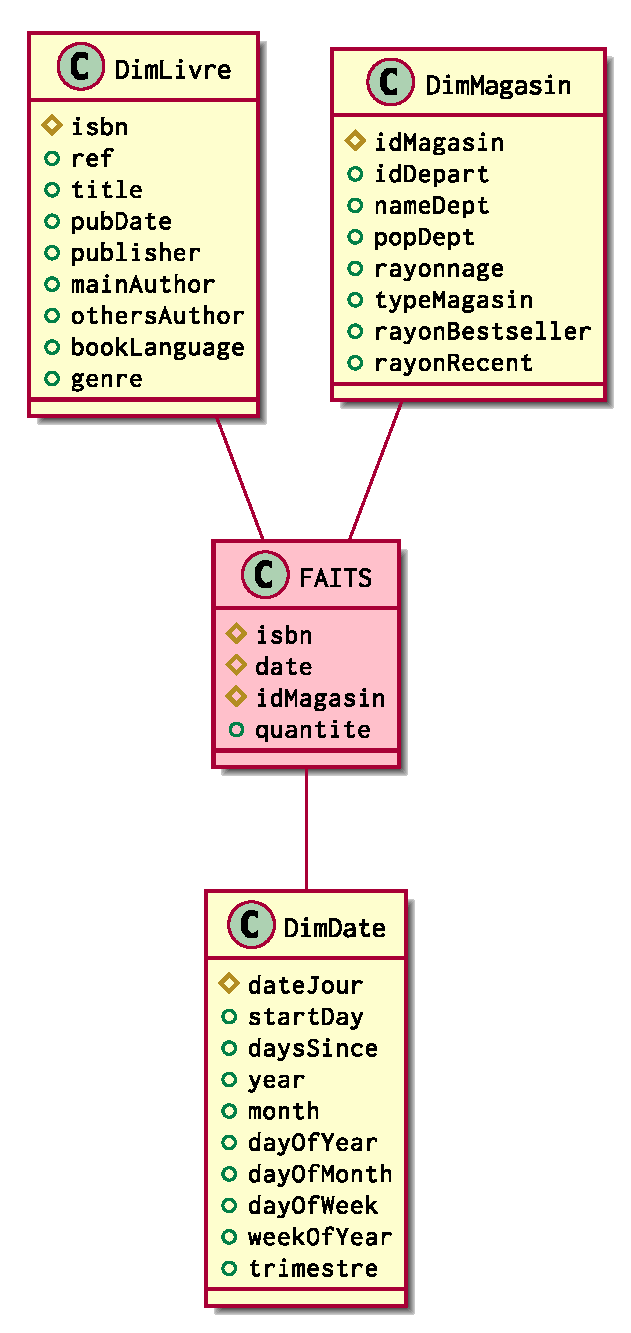
\includegraphics[scale=0.5]{contexte.eps}}
      \caption{Contexte, dimensions et table de faits}
      \label{contexte}
  	\end{wrapfigure}
  	
Lors du premier sujet de TD, nous avons pu modéliser les processus de l'entreprise \textit{Fantastic}. Nous nous sommes sur cette partie concentrés sur l'alimentation de tables dans la bases de données à partir de différentes sources grâce au logiciel \textit{Pentaho Kettle}\footnote{Site officiel de \textit{Pentaho Kettle} : \url{http://www.pentaho.com/product/data-integration}.} dédié à l'intégration de données.\\

Le schéma ci-contre (Figure \ref{contexte}) reprend le \textit{contexte} développé en fin du premier TD dans une version affinée et améliorée.\\

Il a été question dans cette suite de TD de \textit{réaliser l'intégration des différentes dimension afin de construire la table de faits}. Les sections suivantes reprennent de manière concise ce qui a été réalisé  pour l'intégration de chacune des dimensions jusqu'aux jointures finales pour la table de faits.
  	

\section{Dimension Magasin -- \texttt{DimMagasin}}

Une jointure est réalisée entre le fichier \texttt{marketing.ods} et les départements avant d'alimenter une table dans la base de données Oracle.\\

Pour ce faire, une étape de validation est mise en place pour s'assurer que les identifiants des magasins sont bien formatée. Une autre validation est effectuée du côté des départements sur le fichier \texttt{departementsInsee2003-nf26.csv}.

	\begin{figure}[H]
      \centerline{\includegraphics[width=\textwidth]{../TD2/screenshots/screenScriptDimMagasin.png}}
      \caption{Traitement de la Dimension Magasin}
      \label{magasin}
  	\end{figure}
  	
  	Le tout est inséré dans une table \texttt{DimDate} dans le schéma Oracle. La figure \ref{magasin} reprend les traitements effectués pour cette dimension.

\section{Dimension Date -- \texttt{DimDate}}

	Pour la génération de la date, nous avons repris le template proposé par \textit{Kettle}, c'est à dire le fichier \texttt{"Pentaho/design-tools/data-integration/samples/transformations/General - Populate date dimension.ktr"} où \texttt{Pentaho} est le répertoire d'installation du logiciel.\\
	
	Nous avons adapté ce dernier fichier pour qu'il puisse générer des dates sur la même période que celle des ventes ; en particulier, nous avons veiller à retirer les heures et à changer le formatage pour que celui-ci corresponde à ceux utiliser dans la suite. Les données générées ont été stockées dans la table une table \texttt{DimDate}. La figure \ref{date} reprend les traitements effectués pour cette dimension.


	\begin{figure}[H]
      \centerline{\includegraphics[width=\textwidth]{../TD2/screenshots/screenScriptDimDate.png}}
      \caption{Traitement de la Dimension Date}
      \label{date}
  	\end{figure}
  	

\section{Dimension Livre -- \texttt{DimLivre}}

	Pour les produits, il s'est principalement agit de récupérer les données depuis le catalogue disponible en lecture publique sur le schéma \texttt{NF26PROF2}. Les données ont été traitées pour extraire l'auteur principal et répertorier, s'il y en avait, les autres auteurs. La chaîne de caractère \texttt{"0000000000000"} a été choisie comme valeur par défaut pour les ISBN mal formatés. De mêmes, les autres champs ont été corrigés pour intégrer des valeurs par défaut sur les données manquantes. Les données ont été stockées dans la table une table \texttt{DimLivre}. La figure \ref{livre} reprend les traitements effectués pour cette dimension.


	\begin{figure}[H]
      \centerline{\includegraphics[width=\textwidth]{../TD2/screenshots/screenScriptDimLivre.png}}
      \caption{Traitement de la Dimension Livre}
      \label{livre}
  	\end{figure}
  	


\section{Table des faits -- \texttt{Faits}}
	
	Sur la table des faits, il s'est principalement agit de joindre les différentes informations grâce aux clés primaires de chacune des dimensions : \texttt{(isbn)} pour la dimension \texttt{DimLivre} ; \texttt{(idMagasin)} pour la dimension \texttt{DimMagasin} et (\texttt{dateJour}) pour la dimension \texttt{DimDate}. Pour ce faire, nous avons renommé quelques champs pour que cela soit uniformisé en \texttt{camelCase}. Nous avons aussi pris soin de remplacer les données manquantes ainsi:
	\begin{enumerate}
		\item \texttt{"9999999999999"} a été choisie comme valeur par défaut pour les ISBN mal formatés du fichier de ventes \texttt{Fantastic};
		\item Une chaîne de caractère vide (\texttt{""}) a été choisie comme valeur par défaut pour les ID de magasin mal formatés ;
		\item \texttt{"0000-00-00"} a été choisie comme valeur par défaut pour les dates mal formatées ;
	\end{enumerate}

	Des tris ascendants ont été effectués avant d'effectuer les jointures. Après chaque jointure, nous avons veiller à supprimer une clé alors dupliquée puisqu'il s'est agit de faire des jointures internes -- \texttt{"INNER JOIN"} en \textit{SQL}. De même, il s'est agit de réaliser une agrégation de lignes pour compter le nombre de ventes réalisés d'un même produit, le même jour, et dans le même magasin. Les données agrégées ont ensuite été sauvegardées dans une table dans le schéma Orale.\\

	Au niveau de la constitution de la base de faits, nous n'avons utilisé que des jointures internes aux données (\texttt{INNER JOIN} en SQL) mais aurions pu, en prenant du recul, utiliser des jointures externes, à gauche ou à droite, (\texttt{LEFT JOIN} et \texttt{RIGHT JOIN} respectivement en SQL) pour conserver l'intégralité des données. Cela aurait nécessité un un plus de traitement -- en particulier des remplacement de données nulle -- mais aurait sûrement été profitable pour pouvoir ensuite effectuer un traitement sur les ventes pour lesquelles leur contexte n'est pas connu en intégralité. La capture d'écran suivante (Figure \ref{traitementFaits}) reprend les différents traitements des lignes, de leurs importation à leur insertion dans la table de faits.
	
	\begin{figure}[H]
      \centerline{\includegraphics[width=\textwidth]{../TD2/screenshots/screenInsertionFaits.png}}
      \caption{Constitution de la base de faits -- aperçu sur les lignes traitées}
      \label{traitementFaits}
  	\end{figure}

\section{Difficultés rencontrées}

	Durant cette réalisation, nous avons rencontré quelques problèmes, en particulier lorsqu'il s'agissait d'effectuer des conversions. \textit{Pentaho} n'arrivait pas à convertir les ISBN ainsi que les dates malformées -- c'est à dire les ISBN qui ne consistaient pas en 13 chiffres et les dates sous un autre format que le format \texttt{"yyyy-m-dd"}. Cela était dû au fait que les champs étaient considérés comme des tableaux d'octets plutôt que comme des chaînse de caractères. Cela s'est réglé facilement en désactivant la \textit{conversion repoussée} -- « \textit{lazy conversion} » en anglais -- lors de l'importation du fichier CSV \texttt{Fantastic}.\\
	
	Aussi il a été impossible dans certains cas de changer le nom de certaines colonnes car elles n'étaient alors pas reconnues dans la suite. Si ce problème est anodin, il n'a pas permis de finir notre travail de clarification des dénominations que nous voulions parfaire avec le formatage des noms en\textit{camelCase}. Nous avons aussi dû convertir les dates en chaînes de caractère pour effectuer les jointures car nous rencontrions des erreurs.\\
	
	Enfin, il fut difficile de travailler sur nos machines personnelles pour plusieurs raisons en particulier par ce que certaines dépendances ne sont pas installées -- ce qui est normal pour les drivers propriétaires pour les connexions aux bases de données Oracle -- ou parce que certaines sont dépréciées et donc non disponibles sur les dépôts officiel de certaines distributions -- c'est le cas de la librairie \texttt{webkitgtk} qui n'est plus supportée sous \textit{Fedora} 27. Néanmoins, nous avons réussi à résoudre cela avec un peu de débrouillardise.\\
	
	\[ \star \quad \star \quad \star \]
  
\newpage
\nocite{*}
%\bibliographystyle{plain}
\bibliographystyle{unsrtnat}

% Autres styles de bibliographie non utilisés
%\bibliographystyle{abbr}
%\bibliographystyle{alpha}

%\bibliography{biblio} % Affiche la bibliographie
%\newpage
%\includepdf[pages=1-3]{../sujetTP3.pdf}
\end{document}
